\documentclass{article}

% use Times
\usepackage{times}
% For figures
\usepackage{graphicx} % more modern
%\usepackage{epsfig} % less modern
\usepackage{subfigure} 

% For citations
\usepackage{natbib}

% For algorithms
\usepackage{algorithm}
\usepackage{algorithmic}

% As of 2011, we use the hyperref package to produce hyperlinks in the
% resulting PDF.  If this breaks your system, please commend out the
% following usepackage line and replace \usepackage{icml2017} with
% \usepackage[nohyperref]{icml2017} above.
\usepackage{hyperref}

% Packages hyperref and algorithmic misbehave sometimes.  We can fix
% this with the following command.
\newcommand{\theHalgorithm}{\arabic{algorithm}}

% Employ the following version of the ``usepackage'' statement for
% submitting the draft version of the paper for review.  This will set
% the note in the first column to ``Under review.  Do not distribute.''
%\usepackage{icml2017} 

% Employ this version of the ``usepackage'' statement after the paper has
% been accepted, when creating the final version.  This will set the
% note in the first column to ``Proceedings of the...''
\usepackage[accepted]{icml2017}

% Stuff I added %%%%%%%%%%%%%%%%%%%%%%%%%%%%%%%
\usepackage{bm, amsmath}
%%%%%%%%%%%%%%%%%%%%%%%%%%%%%%%%%%%%%%%%



% The \icmltitle you define below is probably too long as a header.
% Therefore, a short form for the running title is supplied here:
\icmltitlerunning{Submission and Formatting Instructions for ICML 2017}

\begin{document} 

\twocolumn[
\icmltitle{Probabilisitic Graphical Models IFT6269 Project \\ 
Latent Dirichlet Allocation}

% you can specify symbols, otherwise they are numbered in order
% ideally, you should not use this facility. affiliations will be numbered
% in order of appearance and this is the preferred way.
\icmlsetsymbol{equal}{*}

\begin{icmlauthorlist}
\icmlauthor{Patrice B\'echard}{equal,um}
\icmlauthor{Th\'eophile Gervet}{equal,mg}
\end{icmlauthorlist}

\icmlaffiliation{um}{Universit\'e de Montr\'eal, Montr\'eal, Canada}
\icmlaffiliation{mg}{McGill University, Montr\'eal, Canada}

\icmlcorrespondingauthor{Patrice B\'echard}{patrice.bechard@umontreal.ca}
\icmlcorrespondingauthor{Th\'eophile Gervet}{theophile.gervet@umontreal.ca}

% You may provide any keywords that you 
% find helpful for describing your paper; these are used to populate 
% the "keywords" metadata in the PDF but will not be shown in the document
\icmlkeywords{boring formatting information, machine learning, ICML}

\vskip 0.3in
]

% this must go after the closing bracket ] following \twocolumn[ ...

% This command actually creates the footnote in the first column
% listing the affiliations and the copyright notice.
% The command takes one argument, which is text to display at the start of the footnote.
% The \icmlEqualContribution command is standard text for equal contribution.
% Remove it (just {}) if you do not need this facility.

%\printAffiliationsAndNotice{}  % leave blank if no need to mention equal contribution
\printAffiliationsAndNotice{\icmlEqualContribution} % otherwise use the standard text.

\begin{abstract} 
TODO
\end{abstract} 

\section{Introduction and Related Works}

\subsection{Latent Dirichlet Allocation}

\subsubsection{Generative Process}
Latent Dirichlet allocation (LDA) is a generative probabilisitic model of a corpus of $D$ documents $\{\mathbf{w}_1,..., \mathbf{w}_D\}$. Each document $\mathbf{w}_d = (w_{d,1},...,w_{d,N_d})$ is a sequence of $N_d$ words from a vocabulary indexed by $\{1,...,V\}$. 

The basic idea behind LDA is that each document is represented as a random mixture over $K$ latent topics, where each topic is characterized by a multinomial distribution over words, parametrized by a vector $\bm{\beta}_{k}$, $k \in {1,...,K}$. 

Formally, LDA assumes the following generative process for each document $\mathbf{w}_d$:
\begin{enumerate}
\item Sample a distribution over topics $\bm{\theta_d} \sim Dir(\bm{\alpha})$
\item For each of the $N_d$ words $w_{d,n}$ independently:
\begin{enumerate}
\item Draw a topic from the distribution over topics $z_{d,n} \sim Mult(\bm{\theta}_d)$
\item Draw a word from this topic \\ 
$w_{d,n} \sim Mult(\bm{\beta}_{z_{d,n}})$
\end{enumerate}
\end{enumerate}
This generative process is illustrated in the directed graphical model of figure \ref{graph_model}.

\begin{figure}[ht]
\vskip 0.2in
\begin{center}
\centerline{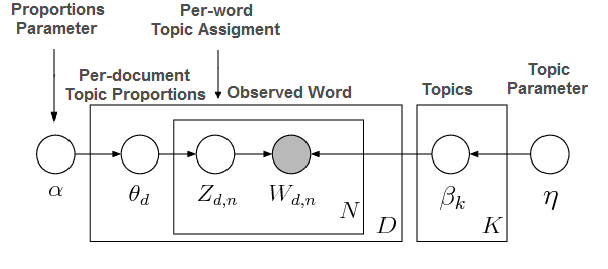
\includegraphics[width=\columnwidth]{LDA_graph_model}}
\caption{Graphical model corresponding to the generative process for LDA.}
\label{graph_model}
\end{center}
\vskip -0.2in
\end{figure} 

The joint distribution associated with this model is:
\begin{multline} 
	\label{joint}
	\prod_{k=1}^{K} p(\bm{\beta}_k | \bm{\eta}) \\
	\prod_{d=1}^{D} p(\bm{\theta}_d | \bm{\alpha})
	\prod_{n=1}^{N_d} p(z_{d,n} | \bm{\theta}_d) p(w_{d,n} | z_{d,n}, \bm{\beta}_{1:K})
\end{multline}
where \\
$z_{d,n} \sim Mult(\bm{\theta}_d)$, i.e $p(z_{d,n} | \bm{\theta}_d) = \theta_{d, z_{d,n}}$ \\
$w_{d,n} \sim Mult(\bm{\beta}_{z_{d,n}})$, i.e $p(w_{d,n} | z_{d,n}, \bm{\beta}_{1:K}) = \beta_{z_{d,n},w_{d,n}}$ \\
$\bm{\beta}_k \sim Dir(\bm{\eta})$ \\
$\bm{\theta}_d \sim Dir(\bm{\alpha})$ \\

This generative process is just a model of the structure we assume to be in our data. In reality, we only observe documents $\mathbf{w}_{1:D}$ and our goal is to infer the underlying topic structure: the topics $\bm{\beta}_{1:K}$, the per document distributions over topics $\bm{\theta}_{d}$, and per document per word topic assignments $z_{d, n}$. 

Since the generative process assumes independence between documents, the probability of the whole corpus decomposes as a product of terms for individual documents. In order to clarify the notation, from now on let us consider equations for a single document $\mathbf{w}$ with $N$ words.

Assuming the Dirichlet hyper-parameters $\bm{\alpha}$ and $\bm{\eta}$ are fixed, we want to infer the posterior distribution:
\begin{equation}
 p(\bm{\beta}, \bm{\theta}, \mathbf{z} | \mathbf{w}, \bm{\alpha}, \bm{\eta}) =
 \frac{p(\bm{\beta}, \bm{\theta}, \mathbf{z}, \mathbf{w} | \bm{\alpha}, \bm{\eta})}{p(\mathbf{w} | \bm{\alpha}, \bm{\eta})}
\end{equation}

Unfortunately, this distribution is intractable to compute because the normalization factor $p(\mathbf{w} | \bm{\alpha}, \bm{\eta})$ cannot be computed exactly. We must use approximate inference to estimate the posterior over latent variables $\bm{\beta}$, $\bm{\theta}$ and $\mathbf{z}$. We will explore both variational inference and Gibbs sampling to solve this problem.

\subsection{Related Works}
TODO

\section{Methods}

\subsection{Variational EM}
To make our life easier, we derive a variational EM algorithm for a slightly simpler graphical model for LDA (the one presented in the original paper). We remove the Dirichlet prior over topics, this corresponds to removing the dependence of the $\bm{\beta}$ plate on the $\bm{\eta}$ random variable (see Figure \ref{graph_model2}, left). By doing so, we lose our ability to smooth topics through the $\bm{\eta}$ parameter.

Assuming the $\bm{\alpha}$ parameter and topics $\bm{\beta}$ are fixed, the posterior for a single document $\mathbf{w}$ now takes the form:
\begin{equation}
p(\bm{\theta}, \mathbf{z} | \mathbf{w}, \bm{\alpha}, \bm{\beta}) =
\frac{p(\bm{\theta}, \mathbf{z}, \mathbf{w} | \bm{\alpha}, \bm{\beta})}
		{p(\mathbf{w} | \bm{\alpha}, \bm{\beta})} 
\end{equation}

This expression is still intractable because of the denominator $p(\mathbf{w} | \bm{\alpha}, \bm{\beta})$. 

Let us motivate a variational EM algorithm by looking at how this intractable posterior comes back to bite us when we try to maximize the likelihood of the observed data. Since the probability of the whole corpus decomposes as a product of terms for individual documents, the log likelihood of the whole corpus decomposes as a sum of terms for individual documents. The log likelihood of a single document $\mathbf{w}$ takes the form:
\begin{equation}
log p(\mathbf{w} | \bm{\alpha}, \bm{\beta}) =
	log \int \sum_{\mathbf{z}} p (\bm{\theta}, \mathbf{z}, \mathbf{w} | \bm{\alpha}, \bm{\beta}) d\bm{\theta} 
\end{equation}

Because of the integral over $\bm{\theta}$ and the sum over $\mathbf{z}$ inside the log, we cannot maximize this objective directly. One common way to solve this problem is the Expectation Maximization (EM) algorithm. We make the following observation:
\begin{align}
log p(\mathbf{w} | \bm{\alpha}, \bm{\beta}) 
&= log \int \sum_{\mathbf{z}} \frac{p (\bm{\theta}, \mathbf{z}, \mathbf{w} | \bm{\alpha}, \bm{\beta}) q(\bm{\theta}, \mathbf{z})}{q(\bm{\theta}, \mathbf{z})}  d\bm{\theta} \\
&= \mathbf{E}_q [log \int \sum_{\mathbf{z}} \frac{p (\bm{\theta}, \mathbf{z}, \mathbf{w} | \bm{\alpha}, \bm{\beta})}{q(\bm{\theta}, \mathbf{z})}  d\bm{\theta}] \\
&\geq \mathbf{E}_q [log p(\bm{\theta}, \mathbf{z}, \mathbf{w} | \bm{\alpha}, \bm{\beta})] + \mathbf{E}_q [log q(\bm{\theta}, \mathbf{z})] \\
&= \mathcal{L}(q, \bm{\alpha}, \bm{\beta})
\end{align}
where we have introduced an arbitrary distribution $q(\bm{\theta}, \mathbf{z})$ over the problematic latent variables $\bm{\theta}$ and $\mathbf{z}$, and the last step follows from Jensen's inequality.

The EM algorithm consists in alternatively maximizing the lower bound $\mathcal{L}$ on the log likelihood with respect to the distribution $q$ (the E-step), and with respect to parameters $\bm{\alpha}$ and $\bm{\beta}$ (the M-step).

One can easily show that maximizing $\mathcal{L}$ with respect to $q$ is equivalent to minimizing $KL(q(\bm{\theta}, \mathbf{z}) || p(\bm{\theta}, \mathbf{z} | \mathbf{w}, \bm{\alpha}, \bm{\beta}))$. A simple solution is thus to set $q(\bm{\theta}, \mathbf{z})$ to be $p(\bm{\theta}, \mathbf{z} | \mathbf{w}, \bm{\alpha}, \bm{\beta})$, the true posterior over latent variables under the model.

In our case, things are not so simple: as we have seen, the posterior $p(\bm{\theta}, \mathbf{z} | \mathbf{w}, \bm{\alpha}, \bm{\beta})$ is intractable. This is were variational inference comes into play. The basic idea is to introduce a parametrized family of distributions over latent variables and phrase inference as an optimization problem. 

We parametrize $q$ as follows, according to the mean field independence assumption:
\begin{equation}
q(\bm{\theta}, \mathbf{z} | \bm{\gamma}, \bm{\phi}) =
q(\bm{\theta} | \bm{\gamma}) \prod_{n=1}^N q(z_n | \bm{\phi}_n)
\end{equation}
where the dirichlet parameters $\bm{\gamma}$ and the multinomial parameters $\bm{\phi}_n$, $n \in \{1,...,N\}$ are free variational parameters. The graphical model corresponding to this parameterization is illustrated in Figure \ref{graph_model2}, right.

\begin{figure}[ht]
\vskip 0.2in
\begin{center}
\centerline{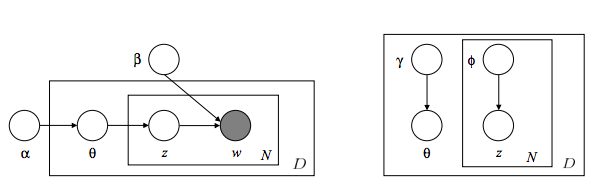
\includegraphics[width=\columnwidth]{LDA_graph_model2}}
\caption{Graphical model corresponding to the generative process for LDA.}
\label{graph_model2}
\end{center}
\vskip -0.2in
\end{figure} 

Now variational inference consists in solving the following optimization problem:
\begin{equation}
(\bm{\gamma}^*, \bm{\phi}^*) =
\underset{\bm{\gamma}, \bm{\phi}}{\text{arg min}}
	KL(q(\bm{\theta}, \mathbf{z} | \bm{\gamma}, \bm{\phi}) || p(\bm{\theta}, \mathbf{z} | \mathbf{w}, \bm{\alpha}, \bm{\beta}))
\end{equation}

Note that $q(\bm{\theta}, \mathbf{z} | \mathbf{w}, \bm{\gamma}^*, \bm{\phi}^*)$ is actually a conditional distribution varying as a function of $\mathbf{w}$ because the optimization objective depends on $\mathbf{w}$. It can thus be seen as an approximation to the posterior $p(\bm{\theta}, \mathbf{z} | \mathbf{w}, \bm{\alpha}, \bm{\beta})$.

With this tool at our disposal, we can come back and complete the EM algorithm described in section 1.1.2. We can expand our variational lower bound on the per-document log likelihood as follows:
\begin{multline}
\mathcal{L}(\bm{\gamma}, \bm{\phi},\bm{\alpha}, \bm{\beta}) = 
\mathbf{E}_q [log p(\bm{\theta} | \bm{\alpha})] + 
\mathbf{E}_q [log p(\mathbf{z} | \bm{\theta})] + \\
\mathbf{E}_q [log p(\mathbf{w} | \mathbf{z}, \bm{\beta})] -
\mathbf{E}_q [log q(\bm{\theta} | \bm{\gamma})] -
\mathbf{E}_q [log q(\mathbf{z} | \bm{\phi})]
\end{multline}
where the first three terms correspond to the expected complete log likelihood under $q$ and the last two terms to the entropy of $q$.

\subsubsection{E-step}
In the E-step, we maximize $\mathcal{L}$ with respect to the variational parameters $\bm{\gamma}$ and $\bm{\phi}$. This corresponds to applying the following update rules iteratively until convergence for each document:
\begin{equation} 
\label{phi_update}
\bm{\phi}_{n,k} \propto \bm{\beta}_{k, w_n} exp\{\Psi(\bm{\gamma}_k)\}
\end{equation}
\begin{equation}
\label{gamma_update}f
\bm{\gamma}_{k} = \bm{\alpha}_{k} + \sum_{n=1}^N \bm{\phi}_{n,k}
\end{equation}
where $\Psi(x) = \frac{\Gamma'(x)}{\Gamma(x)}$ is the digamma function.

Theses updates make sense intuitively. Equation \ref{phi_update} tells us that $\bm{\phi}_{n,k}$, the probability that word $w_n$ is generated by latent topic $k$, is proportional to the probability of drawing $w_n$ from topic $k$ times a quantity proportional to how much the document likes topic $k$ (the dirichlet parameter $\bm{\gamma}_k$). Equation \ref{gamma_update} tells us that the dirichlet parameter $\bm{\gamma}_k$ is equal to the pseudo-count $\bm{\alpha}_k$ given by the dirichlet prior plus the expected count of words picking topic $k$.

\subsubsection{M-step}
For the M-step, we maximize the overall variational lower bound with respect to parameter $\bm{\beta}$. We could also maximize with respect to $\bm{\alpha}$ but we chose to keep it fixed to make things simpler. As said before, the overall log likelihood of the corpus is the sum of the log likelihoods for the individual documents. Likewise, the overall variational lower bound is the sum of the individual variational bounds. 

Maximizing with respect to $\bm{\beta}$ gives the following update:
\begin{equation} 
\label{beta_update}
\bm{\beta}_{k,j} \propto \sum_{d=1}^D \sum_{n=1}^{N_d} \bm{\phi}_{d, n, k}
w_{d,n}^{(j)}
\end{equation}
where we abuse notation and index word $w_{d,n}$ which was a scalar until here as a one hot vector.

Equation \ref{beta_update} also has an intuitive meaning: the probability of word $j$ under topic $k$ is proportional to the expected count under the variational distribution of the number of times word $j$ is assigned topic $k$ across the whole corpus.

\subsubsection{Overall Algorithm}
We implemented a variational "EM flavored" algorithm which we described in detail in the algorithm below. Note that to be strictly an EM algorithm, we should maximize $\mathcal{L}$ with respect to $\bm{\phi}$ and $\bm{\gamma}$ all the way at each E-step. Instead, we alternate a single step of improvement with respect to the variational parameters with one step of improvement with respect to $\bm{\beta}$. Our algorithm has the same guarantee to increase the variational lower bound at each iteration, it is just more convenient to check for convergence only for the overall algorithm instead of for each E-step.

\begin{algorithm}[tb]
   \caption{Variational EM}
   \label{algo}
\begin{algorithmic}
   \STATE {\bfseries Input:} documents $\mathbf{w}_1,...,\mathbf{w}_D$
   \STATE Set $\bm{\alpha}_k = 1 / K$ for all $k$ 
   \STATE Randomly initialize variational parameters $\bm{\gamma}$, $\bm{\phi}$ 
   \REPEAT
   \FOR{$d = 1$ {\bfseries to} $D$}
   \FOR{$k = 1$ {\bfseries to} $K$}
  	\FOR{$n = 1$ {\bfseries to} $N_d$}
  	\STATE $\bm{\phi}_{d,n,k} = \bm{\beta}_{k, w_n} exp\{\Psi(\bm{\gamma}_{d,k})\}$
  	\ENDFOR
  	\STATE normalize $\bm{\phi}_{d,n}$ to sum to 1
  	\STATE $\bm{\gamma}_{d,k} = \bm{\alpha}_k + \sum_{n=1}^{N_d} \bm{\phi}_{d,n,k}$
   \ENDFOR
   \ENDFOR
   \FOR{$k = 1$ {\bfseries to} $K$}
   \FOR{$j = 1$ {\bfseries to} $V$}
   \STATE $\bm{\beta}_{k,j} = \sum_{d=1}^D \sum_{n=1}^{N_d} \bm{\phi}_{d, n, k} w_{d,n}^{(j)}$
   \ENDFOR
   \STATE normalize $\bm{\beta}_k$ to sum to 1
   \ENDFOR
   \STATE 
   \UNTIL{objective $\mathcal{L}$ doesn't improve anymore}
\end{algorithmic}
\end{algorithm}

\subsection{Gibbs Sampling}
TODO

%Once again, we consider a single document $\mathbf{w}$ with $N$ words. Recall that we are interested in the latent topics $\bm{\beta}_{1:K}$, the distribution over topics $\bm{\theta}$, and the per word topic assignments $z_{n}$, $n \in \{1,...,N\}$. 

%We could derive conditional distributions for each of these latent variables, and therefore an LDA Gibbs Sampling algorithm, but we note that both $\bm{\theta}_{d}$ and $\bm{\beta}_k$ can be computed using the topic assignments $z_{d,n}$ which are sufficient statistics. This allows us to integrate out the multinomial parameters and simply sample $z_{d,n}$.

\section{Experiments}
TODO

\section{Results}
TODO

% In the unusual situation where you want a paper to appear in the
% references without citing it in the main text, use \nocite
\nocite{langley00}

\bibliography{example_paper}
\bibliographystyle{icml2017}

\end{document} 


% This document was modified from the file originally made available by
% Pat Langley and Andrea Danyluk for ICML-2K. This version was
% created by Lise Getoor and Tobias Scheffer, it was slightly modified  
% from the 2010 version by Thorsten Joachims & Johannes Fuernkranz, 
% slightly modified from the 2009 version by Kiri Wagstaff and 
% Sam Roweis's 2008 version, which is slightly modified from 
% Prasad Tadepalli's 2007 version which is a lightly 
% changed version of the previous year's version by Andrew Moore, 
% which was in turn edited from those of Kristian Kersting and 
% Codrina Lauth. Alex Smola contributed to the algorithmic style files.  
